%% $Id: introduction.tex,v 1.8 2004/07/02 20:57:36 pwaddell Exp $

\chapter{Introduction to Urban Simulation}

\section{Context and Objectives for Urban Simulation}
Urban systems are becoming ever larger and increasingly complex as urban economies,
social and political structures and norms, and transportation and other infrastructure
systems and technologies evolve\footnote{This chapter is updated from
Waddell, P. and G. F. Ulfarsson. (2004).  Introduction to Urban Simulation: Design and Development of Operational Models.
In Handbook 5: Transport Geography and Spatial Systems, K. Haynes, P. Stopher, K. Button \& D. Hensher eds.  Pergammon Press.}.
Scarce resources make efficiency critically important,
and in a democratic context that involves many stakeholders with conflicting values and
priorities, it is neither feasible nor appropriate to deal with major land use and transportation
policies and investments as isolated choices to be decided by planners or bureaucrats within
the bounds of a single organization.

Mathematical and theoretical models have long been used to attempt to reduce complexity and encode a clear and concise understanding of some aspects of urban structure and transportation, as exemplified by the classic work on the Monocentric Model of the city (Alonso, 1964; Mills, 1967; Muth, 1969).  While the value of theoretical models is facilitating a broad understanding of some underlying principles of urban development and transportation, much of this work remains too simplified in its assumptions and too abstract to be of direct value to agencies needing to inform decisions about specific policies and investments in particular urban settings.

To begin to address more operational needs in planning and policy decisions, computerized models representing urban travel and land use began to be developed and used from at least the 1960's in the United States, with the advent of the Urban Transportation Planning System for travel demand forecasting (Weiner, 1997), and the subsequent work on spatial interaction models for predicting locations of households and jobs across urban landscapes (Putman, 1983), which emerged out of earlier work on the Lowry gravity model (Goldner, 1971).  A separate branch of applied urban modelling developed along the lines of the Input-Output model of the macroeconomy developed to describe the structure of economic flows between economic sectors (Leontief, 1966), adding a spatial component and transportation costs to represent economic and transport flows between zones in a region (de la Barra, 1989; Marcial Echenique \& Partners Ltd., 1995).

The objectives for much of the work on land use and transportation modelling in the United States from the 1960's through the 1980's were focused on the planning problem of determining transportation capacity needs -- mostly focusing on roadway capacity -- to accommodate expected demand generated by predicted land use patterns represented by the spatial distribution of households and jobs within a metropolitan area at some future planning horizon.  Over the 1970's and 1980's, increasing pressure from environmental groups, proponents of transit, and others, led to a substantial shift in policy objectives, reflected in the passage of the Clean Air Act Amendments (CAAA) of 1991 and the Intermodal Surface Transportation Efficiency Act (ISTEA) of 1990.

By 1990, a significant degree of attention had emerged on the effects of transportation improvements on land use changes, the potential for long-term induced demand from highway expansion that might significantly undermine the expanded capacity through additional travel, and increasing environmental consequences in the form of emissions and loss of open space due to stimulation of low-density development at and beyond the urban fringe.  The passage of the CAAA and ISTEA legislation set the stage for lawsuits by the Sierra Club and the Environmental Defense Fund and other environmental groups in the San Francisco Bay area, Chicago, Salt Lake City, and other metropolitan areas, on the grounds that the computerized transportation and land use modelling and planning processes did not adequately account for these complex feedbacks between transportation improvements, land use, and air quality (Garrett and Wachs, 1996).

Simultaneously, the policy environment began to shift towards a more multi-modal approach to transportation, including non-motorized and transit modes, other demand-side policies began to emerge as alternative ways to match capacity to needs, including a range of transportation system management techniques (ramp metering, traffic light signalization, and so forth), travel demand management (ride-sharing, staggered work hours, parking pricing policies, congestion pricing, etc.), and land use policies (jobs-housing balance, urban growth boundaries, transferable development rights, concurrency requirements or adequate public facilities ordinances).  The range of policies and strategies under potential consideration by metropolitan areas to address transportation needs has essentially exploded over the past two decades, from a fairly narrow focus on highway capacity expansion to a multi-modal transportation capacity and demand management and land use policies.  The objectives for operational urban land use and transportation models have consequently grown.

Besides the growing need to test the effects and effectiveness of an ever-more diverse range of land use and transportation policies, and their interactions, pressures on operational modelling have grown from a very different perspective.  From the earliest efforts to develop operational urban models, critics have raised serious concerns about the viability of such models.  Lee's ``Requiem for Large Scale Urban Models'' in 1973 (Lee, 1973) cogently argued that efforts to develop operational urban models had failed, and would likely continue to fail for a variety of reasons ranging from insufficient theory to computational and data demands.  Much of the operational work in urban transportation and land use modelling has been criticized as being too much akin to a ``black box'', meaning that its theory and implementation were not clear enough to an observer attempting to understand and evaluate it.  While some of the criticism was aimed at problems that have since clearly been addressed, such as computational requirements, other concerns, such as insufficient behavioural theory, still require substantial attention and are not widely addressed even in many current operational simulation models.  It is valuable to keep these critiques in mind when examining current and emerging modelling approaches.

Combined with this kind of skepticism on a technical level, growing pressures have emerged on the planning and policy-making arenas to become more open and participatory -- in short, more democratic.  The tradition that has emerged within planning agencies of having technical staff run models to support planning processes, without clear and open access to the models, their assumptions, their theoretical foundation and their practical application, has become very inconsistent with the current context demanding more democratic analysis and decision processes.

In summary, the context and objectives for urban modelling have grown far more complex over the past two decades, and combine to shape the needs for urban model development in ways that are sensitive to a range of land use and transportation policies and their interactions, that build on clear and defensible foundations in behavioral theory, and that facilitate participation in the testing of alternative policy strategies and their evaluation.  These are formidable challenges to address in a satisfactory way.


\section{The Design and Implementation of an Operational Urban Simulation System}

\begin{figure}[htp]
\begin{center}
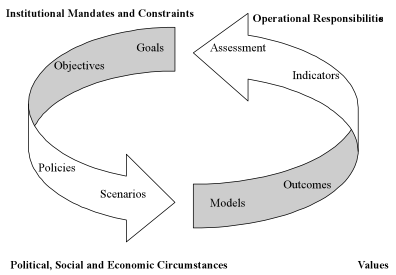
\includegraphics[scale=0.8]{graphics/models-in-process.png}
\end{center}
\caption{Models in the Policy Process}
\label{fig:models-in-process}
\end{figure}

In the balance of this chapter, we explore recent advances and experience in the design and development of urban models that attempt to address these requirements and contextual factors.  General questions of model design and application discussed below are grounded in a case study of the development of the UrbanSim system in the Puget Sound region, and the rationale for each design choice is presented.  UrbanSim has been developed since the late 1990's to address many of the concerns identified above, and represents an ongoing interdisciplinary research development effort to provide operational tools to support the assessment of land use, transportation and environmental policies and plans within metropolitan areas (Noth, Borning and Waddell, 2001; Waddell, 2000; Waddell, 2002; Waddell, et al., 2003).

We propose that models be considered within a broader context in which they will be used to guide or inform policy choices, and that this be considered a participatory and iterative process.  Figure \ref{fig:models-in-process} depicts the proposed policy development process as one that begins with a visioning, or goal-setting phase, and proceeds through development of objectives, identifying policies, formulating policy packages or scenarios, using models to examine the effects of these policy scenarios on important outcomes, and developing indicators and evaluating the effectiveness of the policy scenarios in achieving the original policy goals and objectives.  The process is likely to be iterative for several reasons, chiefly that different stakeholders will disagree about the relative weight to place on each goal, and there may be many possible policy scenarios that could be evaluated.  Ultimately, the process should lead to a convergence of agreement on a set of goals and on the preferred policy strategy for achieving them.  Our hope is that a well-designed policy process that integrates use of models in a participatory decision process will increase the likelihood of a cooperative resolution, as compared to the frequently observed political gridlock now observed in many metropolitan regions.

The model development process we propose is summarized in the following steps:

\begin{enumerate}
\item   Assess the institutional, political and technical context
\item   Assess stakeholders, value conflicts and public policy objectives
\item   Develop measurable benchmarks for objectives
\item   Inventory policies to be tested
\item   Map policy inputs to outcomes
\item   Assess model requirements
\item   Prepare input data
\item   Develop model specification
\item   Estimate model parameters
\item   Calibrate model system
\item   Validate model system
\item   Operational use
\end{enumerate}

Since the focus of this paper is on the design process for developing an operational urban simulation model system, we will cover steps 1-8 in substantial detail and provide only a brief summary of steps 9-12.



\subsection{Assess the institutional, political and technical context}

Who will be using the model system and who will be affected by its use?  What are the institutional mandates and limitations of the organizations involved?  What technical requirements or limitations impose bounding conditions on the problem at hand?  These and related questions logically precede any model development exercise, and set its broad scope and direction.

We use the Puget Sound region in the State of Washington as a case study for clarifying these questions and the discussion that follows.  The federally-designated Metropolitan Planning Organization (MPO) and state-designated Regional Transportation Planning Organization (RTPO) for the region, which contains the major cities of Seattle, Tacoma and Bellevue, is the Puget Sound Regional Council (PSRC).  The PSRC coordinates the development of a Regional Transportation Plan, which is updated every three years, with a major update involving significant model applications every six years.

In 2000, the PSRC commissioned a study to evaluate their current land use and transportation models, and to develop a long-term development strategy for new model development.  The results of this effort are documented in a series of reports (Waddell, et al., 2001; Waddell, Outwater and Bhat, 2001; Waddell, Schroer and Outwater, 2001).  The major planning responsibilities of the PSRC are summarized in Table \ref{tab:responsibilities}, and although the focus of the organization is heavily oriented towards regional transportation planning, it also serves as a regional coordinator of land use plans due to the adoption of a state Growth Management Act (GMA) in 1990.  The PSRC has no direct taxation or operational power other than these planning functions, and local governments still retain full control of land use policies and most transportation investments.  The agency is therefore similar to MPOs in the United States in having relatively little political authority or leverage other than through its role as a regional planning and coordinating agency.

This institutional context influences the planning and design of an operational urban simulation model.  First, it implies a regional scope to the modelling in order to support the primary responsibility of the agency to develop the Regional Transportation Plan.  Second, it implies that there should be a significant degree of involvement and coordination with local cities and counties within the region if the PSRC is to be able to leverage a well-coordinated and effective set of land use and transportation policies and investments.  Third, due to the dispersion of political authority at a local level, especially for land use policies, it suggests that the model system should be designed in a way that is useful to local governments in developing and evaluating land use and transportation policies, so that these policies may be more effectively coordinated across the region.

\begin{table}[htp]
\caption{Major Planning Responsibilities of the Puget Sound Regional Council}
\label{tab:responsibilities}
\begin{tabular}{ p{1.45in}  p{4.4in}  }
\addlinespace
\toprule[1.5pt]
\multirow{6}{1.45in}{Transportation}
& Produce a regional transportation plan (RTP) that will establish the planning direction for regionally significant transportation projects.\\
& Establish regional transportation policy and set minimum standards for state government to integrate into its transportation planning. \\
& Carry out MPO functions (federally mandated):
\squishlist
\item Preparation of an RTP (20-year plan for integrated regional transportation system with both short and long-term actions)
\item   An annual work program
\item   Collaborative planning program with Washington State Department of Transportation (WSDOT), transit operators and air quality agencies
\item   Three-year Transportation Improvement Program (TIP)
\squishend \\
& Carry out RTPO functions (state mandated):
\squishlist
\item   Preparation of an RTP
\item   Six-year capital plan
\item   Certify that transportation elements of local comprehensive plans are consistent with the regional transportation plan
\item   Certify that transportation elements of county, city and town comp. plans are consistent with state comprehensive planning law
\item   Assure that the region's transportation projects are consistent with the RTP
\item   Manage right-of-way preservation proposals for high-capacity transportation development, in conformance with the RTP and other regional strategies
\item   Work with WSDOT to plan corridor transportation strategies
\squishend \\
& Determine categories of priorities for the region among recommended regionally significant transportation projects. \\
& Review and comment in the federal and state environmental impact assessment process (NEPA\/SEPA) on proposed actions with potential significant impact on the implementation of the RTP. \\
\midrule
\multirow{3}{1.45in}{Growth Management} & Maintain VISION 2020 (PSRC, 1995) and updates as the regional growth management strategy.\\
& Develop multi-county planning policies.\\
&   Coordinate local and regional growth management planning efforts.\\
\midrule
Countywide Comp. Plans   & Review all countywide plans for consistency with the adopted regional growth and transportation strategy.\\
\midrule
\multirow{4}{1.45in}{Regional Data Base Development}
&   Support development of the RTP and regional growth management.\\
&   Forecast and monitor economic, demographic, and travel conditions.\\
&   Develop data base jointly with relevant state agencies.\\
&   Respond to data prepared by Washington Office of Financial Management.\\
\midrule
\multirow{2}{1.45in}{Technical Assistance} &    Provide technical assistance to local and state governments.\\
&   Provide general planning assistance to small cities and towns.\\
\midrule
Discussion Forum & Provide a forum for discussion among local and state officials and other interested parties.\\
\bottomrule[1.5pt]
\multicolumn{2}{l}{Source:  PSRC Interlocal Agreements 1981, 1998, cited in Waddell, Schroer and Outwater, 2001}\\
\end{tabular}
\end{table}


A significant aspect of urban planning and policy in the U.S. context, particularly in the Pacific Northwest, is the degree of involvement by community and advocacy groups in the planning process.  In Portland, Oregon, a well-documented process was spearheaded by grass-roots environmental activists who opposed a proposed circumferential highway around Portland that they argued would lead to further low-density development and more auto use.  The Land Use, Transportation and Air Quality Connection (LUTRAQ, 1993) process involved environmental groups and other community advocates in the metropolitan planning process and led to the development of alternative policy scenarios that were more transit oriented and involved the use of land use policies to concentrate development around transit stations.  Ultimately, in this case, the scenario proposed by LUTRAQ proved to be persuasive, and the highway project was abandoned.

In the Puget Sound, there are many non-profit agencies representing advocacy interests, such as protecting the environment (Sierra Club, Northwest Environment Watch), for promoting non-motorized transportation alternatives (Transportation Choices Coalition), promoting growth management (1000 Friends of Washington), arguing against the regional transit agency (Sound Transit) light rail plans (Sane Transit) and for road expansion (Citizens for Mobility), and organizations promoting limitations in governmental taxing authority and spending (Permanent Offense).  In this populist context, in which the process often receives as much attention as the outcome, the development of a model system for regional planning of transportation investments and land use policies must be attentive to the active role of the public participation, and the many diverse stakeholders and values that must be recognized as an integral part of the process of planning and decision making in the region.

\subsection{Assess Stakeholders, Value Conflicts and Public Policy Objectives}

As should be clear from the forgoing discussion, there are many stakeholders involved in regional planning and decision making in the Puget Sound region as well as in metropolitan areas elsewhere in the U.S. and abroad, and that they often hold conflicting values over community priorities.  Some of these conflicts arise from NIMBYism (not in my backyard), a pattern of resistance to location decisions in which parochial self-interests weigh against broader regional objectives.  Many other conflicts are over more fundamental differences in values, such as how important it is to move cars faster on the roadways as compared to preserving forest and agricultural lands, or increasing the affordability of the housing in the region, or promoting economic growth.  In the Puget Sound, efforts to bring these diverse interests and perspectives together to develop a consensus around a long-term vision for the region were coordinated by the PSRC, culminating in a document called Vision 2020 (PSRC, 1995).  This process is being updated in 2008, with a new target of 2040.  In other regions similar visioning efforts have been carried out by non-profit organizations or coalitions of public and private organizations, such as the Envision Utah process in the Greater Wasatch Front region of Utah.  Vision 2020 presented a consensus on four major themes for policy development (the following excerpts are from PSRC, 1995):

\begin{itemize}
\item   Improve efficiency through effective transportation system management. The strategy places the highest priority on maintenance and preservation of all elements of the transportation system: roads, transit, ferries, freight and goods, and non-motorized.
\item   Use transportation demand management measures to reduce travel demand, provide new sources of revenue, and help meet environmental objectives.  In the short term, the region will pursue incentives to encourage transit use, ridesharing, bicycling, walking, and telecommuting. In the long term, the region will study and consider transportation pricing strategies to generate revenue for system improvements, provide incentives for travel outside of peak periods, and discourage the growth of driving alone.
\item   Focus transportation investments to support transit and pedestrian-oriented land use patterns. Serving compact communities with high quality transit service and locating bus stops near residences are examples of effective ways to reduce the need for motor vehicle use.
\item   Add transportation capacity where appropriate to provide alternatives to automobile travel, enhance safety and access, and improve freight and goods mobility. The strategy stresses the importance of system planning for non-motorized and transit facilities and services, so that these enhancements can be programmed similar to street and highway improvements rather than occurring in a piecemeal fashion. Improvements to the road network to provide a more comprehensive and connected roadway system are also called for.
\end{itemize}

The value of a coordinated and participatory visioning process such as Vision 2020 or Envision Utah is that it elicits from a diverse set of stakeholders a broad sense of shared values that can help set the stage for developing politically viable strategies for action, and avoiding political impasse or legal confrontation.  Increasingly, the environmental movement in the U.S. has found a viable strategy in legally confronting MPOs and state departments of transportation over planned highway projects, arguing under the Clean Air Act Amendments that the secondary effects of the highway projects on land use and air quality were not adequately assessed, and the courts have frequently agreed.  Several lawsuits around the country have documented that this strategy can be successful in blocking major highway projects.  In order to avoid such legal impasse, regional visioning and planning efforts must reach out to environmental groups and other stakeholders representing a range of diverse values and perspectives.  The implications for model development are significant.  Models will be heavily questioned by skeptical stakeholders, and should be made as transparent in their design as possible.  Ideally, the full range of stakeholders should be involved in the process of designing and implementing models in order to ensure that the design avoids any significant biases that favor one stakeholder perspective over another.  This would decrease the likelihood of a legal challenge being made in the first place, and decrease the likelihood that such a legal challenge would be successful.  The recent emergence of a Value Sensitive Design methodology in information technology can be productively applied to the development and design of complex urban simulation models (Friedman and Kahn, 1994; Friedman, Kahn and Borning, 2002).

\subsection{Develop measurable benchmarks for objectives}

Once policy objectives are identified, even while there remains significant difference of perspective over their relative priority, it is possible and quite useful to begin to develop measurable benchmarks for evaluating progress towards these objectives.  If there are thresholds that are relevant due to federal, state or local requirements, such as for air quality, these provide clear and measurable targets for achieving policy objectives.  In other cases, such as transportation efficiency, it may be much more difficult to obtain consensus around a set of benchmarks that should be attained, or even what measures should be used to represent progress.  For example, there may be significant differences of opinion over what levels of service on the roadways are acceptable, or whether multi-modal levels of service should be used instead.  There is also little agreement about whether mobility (efficiency in moving from one location to another) or accessibility (ease in reaching desired activities) should be the guiding principle for transportation policy.   These two approaches yield very different strategies for intervention, with the former focusing on expansion of roadway capacity and the latter on mixed modes and coordinated land use policies.

Unfortunately, this phase of planning is too often either ignored or left ambiguous, providing insufficient support for later stages in the process.  A preferred approach would be to establish clear benchmarks where possible, and at the least develop clear measures that indicate the direction of progress on each objective.  These measures should then form the basis for indicators that are used in evaluating alternative policy strategies after developing and implementing the model system and using it to compare a baseline and alternative policy scenarios.  We will return to this topic later in the description of the process.

\subsection{Inventory Policies to be Tested}

The following inventory (see Table \ref{tab:policies}) of policies is an incomplete but representative list of the types of policies under consideration in many metropolitan areas that affect or are affected by land use and transportation choices.

\begin{table}[htp]
\caption{Policies to be Potentially Evaluated}
\label{tab:policies}
\begin{tabular}{ p{1.45in}  p{4.4in}  }
\addlinespace
\toprule[1.5pt]
\multirow{5}{3cm}{Transportation Capacity}
&   Expansion of roadways\\
&   Expansion of fixed-guideway transit systems\\
&   Expansion of bus transit systems\\
&   Expansion of high-occupancy vehicle lanes\\
&   Expansion of bicycle and pedestrian facilities and amenities\\
\midrule
\multirow{4}{3cm}{Transportation System Management}
&   Highway ramp metering\\
&   Incident response systems\\
&   Traffic signalization\\
&   Traffic calming measures\\
\midrule
\multirow{4}{3cm}{Transportation Demand Management}
&   Incentives for carpooling/vanpooling\\
&   Incentives for staggered work hours\\
&   Parking pricing\\
&   Congestion pricing\\
\midrule
\multirow{7}{3cm}{Land Use/Growth Management Policies}
&   Urban growth boundaries\\
&   Concurrency requirements or adequate public facilities ordinances\\
&   Comprehensive land use plans\\
&   Zoning\\
&   Promoting urban designs such as neo-traditional neighborhood design\\
&   Transit-oriented development\\
&   Transferable development rights\\
\midrule
Incentives for infill and redevelopment &
    Development impact fees\\
\midrule
Economic Development Policies &
    Property tax abatements, incentives for business or real estate development\\
\midrule
\multirow{2}{3cm}{Environmental Policies}
&   Protection of environmentally sensitive or hazardous areas\\
&   Air quality conformity measures\\
\bottomrule[1.5pt]
\end{tabular}
\end{table}

Many other policies could be potentially included for analysis, and each one would require an assessment of its impact on the model design.  Some policies may impose significant costs on the model development effort in order to effectively address them, but fall fairly low on a prioritization of policies to test.  In such cases, it may be appropriate to drop the policy from further consideration, recognizing this as a design choice.

\subsection{Map Policy Inputs to Outcomes}

For each of the policies to be considered, there is some a priori expectation, or range of expectations, about how the policy would affect outcomes that are intended, and others that may be indirect effects.  The conceptual mapping of policy inputs to outcomes should be informed broadly by theory within the social and natural sciences.  We cannot adequately describe within the scope of this paper the relevant theoretical foundations for this activity, and the reader is referred to other sources to elaborate on the treatment here (DiPasquale and Wheaton, 1990; Waddell and Moore, 2001).

Figure \ref{fig:markets} portrays at a general level the broad scope of interactions among households, firms, developers and governments within markets for real estate, labor, and goods and services.  Developers use land to construct housing and nonresidential floor space that are demanded by households and businesses, who are also interacting in the labor market and the markets for goods and services.  Governments provide infrastructure and services, regulate and in some cases alter prices for the use of land and infrastructure.  This general framework provides a point of departure for considering the effects of alternative governmental policies and investments.

The key agents that generate or respond to the policies outlined are households, individuals, employers, developers, and governments. Households make a cluster of interdependent long-term lifestyle choices, including when to move, neighborhoods to locate within, the type of housing to rent or purchase and the number of vehicles to own (Salomon, Waddell and Wegener, 2002). Individuals within households choose their labor force and educational status, their job mobility and job search, their daily activity schedule, their transportation mode and route. Employers choose to start and close establishments, and choose site locations, size of employment, and types and quantities of real estate to rent or purchase. Developers choose to undertake real-estate development projects, and the scale and locations of those projects. Governments set policies and make investments that affect the choices of other agents, and also make development choices regarding public facilities, including type, location, and scale of development.

\begin{figure}[htp]
\begin{center}
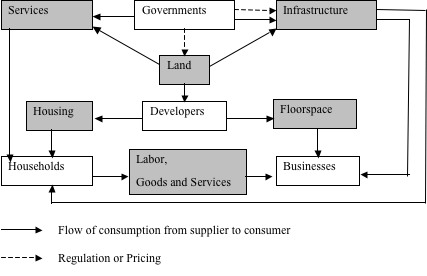
\includegraphics[scale=0.8]{graphics/markets.png}
\end{center}
\caption{\label{fig:markets}{Linked Urban Markets}}
\label{fig:markets}
\end{figure}

The agents, choices and interactions that we suggest are appropriate to connect a broad range of policy inputs to outcomes are summarized in Figure \ref{fig:data-model}.  We suggest that governmental actions such as regulations and infrastructure investments be treated as exogenous, if the objective of the modelling is to evaluate alternative public policies.  The other choices and processes depicted lead to logical structures for model components, and the representation of agents and objects on which they act.

For each of the policies identified, it should be possible to trace the expected causal paths from policy input to outcomes, and this conceptual mapping should provide a foundation for developing a model design that will be responsive to the policy in question.  Although there is insufficient space available to do this systematically for those policies listed in Table 2, we present one example and the reader is left to consider how this might be applied to other policies.

\begin{figure}[htp]
\begin{center}

\includegraphics[scale=0.8]{graphics/data-model.png}
\end{center}
\caption{\label{fig:data-model}{Agents, Choices and Interactions to Represent in a Complete Urban Model}}
\end{figure}


Consider the example of the imposition of an Urban Growth Boundary (UGB).  The intent of such a policy is to encourage compact development within the boundary, and limit urban development outside the boundary, in order to protect farm and resource lands from urbanization and to promote more efficient use of existing infrastructure.  Critics argue that it also leads to rapid housing price inflation.  How, and to what extent, does the UGB produce these outcomes?   First, it should be noted that the UGB is actually not a direct regulatory policy that is implemented independently of other policies.  It is actually a higher-order policy that must be implemented through changes in the comprehensive land use plans of cities and counties affected by the boundary, in order to make those plans consistent with the intent of the UGB.  In other words, these local jurisdictions may be required by state law first, to delineate a UGB, and second, to change their land use plans and zoning to downzone the areas outside the UGB to an agricultural intensity, and to upzone the areas within the UGB in order to increase the intensity of land use and to accommodate anticipated development over a planning horizon.  In Washington, the UGB is intended to include sufficient developable area to accommodate 20 years of development, and is to be revisited and extended when it no longer contains sufficient area to accommodate this level of anticipated development.

In practical terms, the intent of the UGB policy is operationalized through land use plans and zoning and coordinated with other infrastructure choices and land use policies, so the model must be made sensitive to these policies if it is to be sensitive to UGB policies.  Second, the effects of the UGB policy on prices are uncertain, since there are competing forces at work.  On the one hand, the UGB policy and the resulting downzoning of areas outside it clearly limit the supply of land for future development.  On the other hand, the UGB is to be delineated so that it contains 20 years of development potential, and there are counter-balancing upzoning policies within the UGB.  So the effect of the policy on prices is theoretically ambiguous, and the model would need to be sensitive to the effects of a relative scarcity of land for development, at different levels of intensity of zoning.  Furthermore, there may be indirect effects on household location choices, with the UGB creating a scarce amenity of access to open space for those that would live near the interior border, or in the existing housing that was developed outside the UGB before the policy went into effect.

\subsection{Assess Model Requirements}

Review of background documents provided the foundation for much of the institutional context for model development in the Puget Sound (Waddell, Schroer and Outwater, 2001).  This was augmented by an extensive review of the literature on operational land use and transportation models (Waddell, et al., 2001).  Based on these materials and on extensive interviews with PSRC staff, and surveys of staff in local governments, the Washington State Department of Transportation and several
advocacy groups, the following requirements emerged for new land use and transportation model development at the PSRC (Waddell, Outwater and Bhat, 2001):

The model system must:
\begin{itemize}
\item   Be sensitive to the effects of transportation pricing policies on both travel behavior and land use.
\item   Be able to address the impacts of proposed land use and transportation policies on housing affordability.
\item   Be able to support the role of the Regional Council in monitoring development and compliance with the objectives of VISION 2020 and the Growth Management Act.
\item   Be sensitive to policies that are designed to promote densification, infill and redevelopment., and to the effects of land use policies such as comprehensive land use plans, zoning, and the Urban Growth Boundary on real estate development and the location of households and firms.
\item   Be able to assess policy effects over periods ranging from less than 5 years to 30 years.
\item   Be designed to support a participatory policy process that includes activities such as VISION 2020, where scenarios are generated and publicly discussed.  Public access to the model assumptions, theory, structure, and results is required, and the models must be explainable to a non-technical audience.
\item   Support the creation of performance indicators and evaluation measures suitable for use by the Regional Council in evaluating alternative policy scenarios using, at a minimum, Least Cost Planning and Cost Benefit Analysis techniques.
\item   Be based on an activity-based framework in order to adequately represent the complexity and constraints of travel behavior, and the influence of land use and transportation policies on travel behavior.
\item   Allow comparison of different transit modes, for example rail vs. bus.  The new model system must be capable of adequately representing non-motorized travel behavior.  The model must allow comparison of different auto modes of travel, for example high occupancy vehicles with 2 or 3+ person vs. single occupancy vehicles.
\item   Recognize the impact of land use patterns on demand for transportation.
\item   Allow analysis of demand induced by transportation system improvements.
\item   Be able to assess the impacts of environmental regulations that affect the development of environmentally sensitive lands, such as Salmon habitat, wetlands, floodplains, seismic areas, steep slopes, and other sensitive lands.
\item   Be able to assess the impacts of commute trip reduction and TDM policies, such as different work arrangements (flexible versus fixed work schedule, telecommuting or not, compressed work week or regular work week).
\item   Recognize the effects of multi-modal transportation system and policy changes on real estate development and the location patterns of households and firms.
\item   Be sensitive to the effects of urban design elements such as mixed land use, density, street pattern, transit service and pedestrian amenities on household and firm location and travel behavior.
\item   Be able to analyze the residential movement and location choices made by households, and the influence on these choices of relevant housing and location characteristics.  The model system must be able to model the choice of household members to participate in the labor market, and to choose a work location.  The model system must be able to model the vehicle ownership choices of households.
\item   Be able to analyze the interactions between household choices related to residential mobility and location, labor market participation and workplace, vehicle ownership, and daily activity and travel scheduling.
\item   Be able to represent demographic processes such as the change in household size and structure, and the ageing of the population.
\item   Incorporate a component to model the process of real estate development, including infill and redevelopment, and the effects of various policies on this process.  The new models must distinguish between important types of real estate that are relevant to the goals and objectives of Vision 2020, including adequate representation of different nonresidential, residential, and mixed-use types.
\item   Be able to support the analysis of Transit Oriented Development (TOD), including real estate development, household and business location, to assist in station area planning.
\item   Incorporate a macroeconomic component to model economic growth in the region and its relationship to internal and external economic drivers.  Analyze the factors and policies influencing the location choices and real estate demands of different firms in different industries.
\item   Address freight and commodity transport within and through the region.
\item   Address modal choices and tradeoffs of moving goods by truck, rail, barge or air.
\item   Be able to produce multi-modal travel assignments for roadway, transit and possibly non-motorized systems.
\item   Contain information pertinent to Commute Management Systems (CMS) policies such as workplace incentives, telecommuting, and a greater breakdown of carpool sizes.  The model should provide information showing the effects of Transportation System Management (TSM) initiatives.
\item   Provide output relevant to policies instituted as part of Intelligent Transportation Systems (ITS) such as incident management systems or public information distribution.
\item   Be developed in a way that supports open and unrestricted access to the software by Regional Council staff, consultants, and constituents, in order to maintain and modify the models to meet emerging needs over time.  The model system should support distributed access and use by Regional Council member governments, and should use consistent data for Regional Council and member agency applications.
\item   Be manageable from the perspective of its data requirements.
\item   Have reasonable performance, in terms of computational efficiency, so that an entire run of the full land use and transportation model system can be accomplished within one working day.
\item   Provide tools to facilitate visualization of model results and comparison of scenarios in ways that are useful to non-technical audiences.  The model must provide forecasts of system characteristics tracked by state benchmarks, for example, the benchmarks identified by the State of Washington's Blue Ribbon Commission on Transportation.  The model system must produce output that allows analysis of the best mix of transportation investments.
\item   Allow Multi-Modal Cost-Benefit Analysis, to enable model users to make more informed transportation investment decisions.
\item   Address uncertainty in the models and produce ranges of values for outputs rather than specific results to avoid suggesting artificial accuracy.
\end{itemize}

\subsection{Make Preliminary Model Design Choices}

Having reviewed the context, policy applications and requirements for model development, the stage is set for examining the design choices in more detail.  In the balance of this paper, we explore the design choices and process for developing an operational urban simulation model that satisfies the requirements discussed in the preceding sections.  As design options are discussed, the choices actually made in the design of UrbanSim to address such requirements will be explained, and the discussion will alternate between general topics of model design and specifics of these design choices within UrbanSim.

There are several major design choices that must be considered for an urban simulation system, and the combination of these choices narrows the choice of modelling approach.  The design choices we consider here are the level of behavioral aggregation, the level of determinism, their temporal representation, and the resolution of agents, space, and time.

\emph{Behavioral Resolution}.  The system can work on an aggregate scale of average behaviors or on the disaggregate level of behavior of individual agents. The simulation system can be deterministic or stochastic. Deterministic systems are based on predetermined rates of change and static functions, and the same inputs will always produce the same results. Deterministic models are typically used along with aggregate scale of behavior, since the average behaviors can often be approximated with a fixed rate of change.  But, agent based simulations can also easily be deterministic, for example queuing models, or choice models that force the agents to choose the most likely result.  Stochastic models, on the other hand, contain an element of randomness. Stochastic models typically predict the probability of certain outcomes, and then select one of these based on a procedure that involves drawing a random number and comparing it to the probability distribution of the alternative outcomes.  Alternatives with higher probabilities are proportionately more likely to be selected.

\emph{Resolution of Agents, Space, and Time.}  The size of the units of analysis, or resolution, of the system is another major design decision. Simulation systems range from macroscopic to microscopic in resolution. Macroscopic systems have the largest units of analysis, typically aggregate values for geographic zones, household distributions, or groups of vehicles. These models are in wide use, mostly because they have relatively low computational needs. They run relatively fast and use relatively little memory. Macroscopic models also require much less data than finer resolutions, and the data is more readily available through census data or other such large databases. Macroscopic models are typically static and deterministic.

Microscopic models have a small unit of analysis, for example a single individual, household, vehicle, trip or activity. Microscopic models are being actively developed because their requirements for considerable computational power are increasingly being satisfied by personal computers, making these models more feasible, and they support clearer behavioral specifications than macroscopic models. Microscopic models are typically stochastic, disaggregate models that require enormous amounts of data. The data needs of microscopic models are still a limitation since detailed data on individuals are expensive to collect. Methods to synthesize households from census data exist (Beckman, Baggerly and McKay, 1995) and such methods facilitate the creation of synthetic households for use in micro-simulation.

Mesoscopic models are a mixture of macroscopic and microscopic models. They may use small decision makers but large time steps, or small time steps for large units of analysis. They therefore allow the use of aggregate data for certain aspects of the model but make use of greater detail where it is available.

\emph{Level of Determinism.}      Stochastic models are based on probability distributions. They are most typically used with agent-based simulations in the form of probabilistic choice models. They allow the agent to randomly choose an alternative, which means an agent can end up with an unlikely choice. These models will generally not give the same result if run twice, but the results can be made repeatable by fixing the random seed that controls the random distribution. Such a feature does not make the model deterministic, since it is always probabilistic what happens if the initial condition is changed slightly.

\emph{Temporal Representation.}  Models can also be cross-sectional or dynamic in their representation of time. Cross-sectional (sometimes referred to as static or equilibrium) models are not time dependent, and model conditions are fixed at a hypothetical condition generally identified as a long-term equilibrium. Equilibrium models assume that the system begins in equilibrium and adjusts completely to some exogenous shock, that is, it reaches a new equilibrium. The assumption of equilibrium usually allows the explicit derivation of the solution describing the system, although the underlying functions may be time-dependent. Dynamic models make no assumption about equilibrium, but concentrate on adjustment processes over real calendar time. The solution describing such a model is therefore often impossible to derive analytically and the system must typically be simulated to find the result.

\emph{System Interaction.}  There are complex interactions between components within the urban system that must be represented in any complete urban simulation system, such as the endogenous relationships between land use, transportation, and the environment. Urban simulation systems must therefore either explicitly model the interactions between land use, transportation, and the environment, or interface with separate transportation or environmental models.

This interaction, or interface, between systems is made especially complex because of the different time scales of urban development, transportation, and environmental changes. In particular, there is a large contrast between urban development and transportation. Simulations of urban development work on time scales from a year down to a month, while transportation simulation systems are on the scale of days down to seconds. Environmental models can be on both scales, for example, the effect on wildlife habitat works on the urban development time scale, i.e. years or months, while models of pollution will be on the transportation model scale.

\subsection{Select Modelling Approach}

The modelling approach is a major design decision, though it will be heavily constrained by the preceding design choices.  Several different urban modelling approaches have been developed and applied to either planning or research objectives over the past several decades, and after a hiatus of almost two decades in the U.S., there is now an active and rapidly growing array of research activities developing and deploying new modelling approaches.  Three of these methods were used in the earliest operational urban models, dating from the 1960's and 1970's: spatial interaction, spatial input-output, and linear programming.  Microsimulation was developed in the 1960's, but not applied to urban modeling until the 1980's.  Since the 1980's, the development of discrete choice modeling and the emergence of cellular automata and multi-agent simulation techniques have created a proliferation of modeling approaches.  We discuss each of these approaches below, and the supporting role of Geographic Information Systems and the integration of several of these approaches in the design of UrbanSim.  The review specifically does not cover theoretical advances such as those that have arisen in the form of the new economic geography (Fujita, Krugman and Venables, 1999), that have not been incorporated into operational planning models that are the focus of this paper.

\emph{Spatial Interaction.}  Models based on the spatial interaction approach include some of the earliest efforts to model systematic spatial patterns of urban land use.  The approach draws on the model of gravity in physics, which indicates that gravitational pull increases in proportion to the mass of two objects in space, and decreases with the square of the distance separating them.  Applied to urban settlements and travel, the gravity model implies that travel between two zones increases with the amount of activity in the origin and destination zone, and decreases with the square of the travel impedance between them.  The basic model has been extended to model trip destination choices, residential location choices, and employment location choices (Putman, 1983). This type of model tends to be limited in the degree of spatial detail used, and does not represent many behavioral factors influencing location choices, nor does it represent the role of real estate markets and prices.

\emph{Spatial Input-Output.}  The spatial input-output framework extended the input-output model developed to represent the structure of the U.S. economy (Leontief, 1966) to address spatial patterns of location of economic activity within regions, and the movement of goods and people between zones. For examples of complete urban models based on this approach, see (de la Barra, 1989; Marcial Echenique \& Partners Ltd., 1995).  Zones are treated in a sense as economies that engage in production, consumption, import, and export within the zone and with all other zones in the model.  These economic exchanges between zones are denominated in monetary units, and driven by demand for exports.  Monetary flows are converted to flows of goods and services by type of vehicle, and of commuting and shopping trips by mode.  The approach includes explicit real estate and labor markets, as well as travel demand modelling, and is structured to generate a static equilibrium solution to changes in one or more inputs.  Zone sizes in operational applications tend to be large relative to zone sizes used in typical urban travel modelling.

\emph{Linear Programming.}    Linear programming models of land use are rare. TOPAZ (Dickey and Leiner, 1983), developed in Australia, and POLIS, applied in the Bay Area (Prastacos, 1985) are examples of models that use this approach.  Linear programming optimizes a global objective function, such as consumer surplus or utility, across the entire model system.  The approach is therefore more suited to exploration of alternative land use configurations that might optimize transportation flow, than to reflect realistic behavioral responses to changes in the transportation system or in land use policies.

\emph{Microsimulation.}  Microsimulation as an approach essentially implies a model that is applied at the level of the individual.  Developed in the late 1950's and early 1960's, the method was initially applied to study the effects of social and economic policies (Orcutt, 1957; Orcutt, et al., 1961).  It has more recently been applied to the formulation of urban models such as MASTER (Mackett, 1992), DORTMUND (Wegener, 1985), and UrbanSim (Waddell, 2002).  Microsimulation models used for socio-economic (non-spatial) policies such as taxes are used with a sample of households, and compute the effects of the tax policy alternatives on the sample of households to study distributional, or equity, effects.  Urban, spatially-explicit models, have used combinations of discrete-choice models and transition rates, to predict changes in the state of individuals or households, such as entering or leaving the labor force, and their choices such as residence location.  Once considered too data-intensive, these methods have been growing in popularity because they allow modelling at an individual level, where behavioral theory is clearer, and due to increased interest in detailed characteristics of households for equity analysis and other reasons, can make individual-level analysis more efficient than cross-classification of households using multiple characteristics.

\emph{Discrete Choice.}  Discrete choice modelling techniques are widely used in travel demand modelling, mostly in the analysis of mode choice.  Discrete choice models have been used in some form for much of the last 100 years.  However, it was Daniel McFadden's Nobel-prize winning Random Utility Theory work and his derivation of the generalized extreme value class of models (which includes multinomial and nested logit models) that gave these models a firm foundation within econometrics, and they have since become standard methods in developing models that attempt to predict individual choices among a finite set of alternatives (McFadden, 1973; McFadden, 1984; McFadden, 1981).  Discrete choice models are generic in the sense that they do not impose overly-restrictive assumptions on the choice process, and have been shown capable of addressing large and complex choice sets effectively (Ben-Akiva and Lerman, 1985).  Discrete choice techniques can be readily used in conjunction with other simulation approaches, such as microsimulation.

\emph{Rule-Based.}  Several land use models have been developed in recent years using GIS and a rule-based set of procedures to allocate population, employment, and/or land use.  Examples include the CUF model (Landis, 1994), Uplan (Johnston, 2003) WhatIf? (Klosterman, 1999).  Such rule-based applications may have a useful role in making models more accessible, but there is a risk that model users would interpret the models as having a more behavioral basis than their rules actually contain.  There are also rule-based methods that are emerging from the field of artificial intelligence, using observed data to generate clarification trees of behavioral rules that are used in microsimulation, such as the Albatross activity-based travel model (Arentze, Hofman and van Mourik, 2000).

\emph{Cellular Automata.}  Cellular automata (CA) models have emerged within the broad field of complex systems as a means of representing the emergent properties of simple behavioral rules applied to cells within a grid (Wolfram, 1984).  The approach has now been widely applied to urban land cover or land use change (Benati, 1997; Clarke and Gaydos, 1998; Couclelis, 1997; White and Engelen, 1993).  To date, applications have been principally for research purposes rather than operational planning or policy, though efforts are underway to make these models useful for planning purposes.  The approach is particularly useful for representing the interactions between a location and its immediate environment, but tends to reflect a fairly abstract representation of agents, decisions, and behavior, since the models focus on simulating the change in state of individual cells.  In addition, challenges remain in reconciling the emergent behavior of cells acting on localized rules with more systemic or macro-scale behavior, in validating these models using observed data, and in computational requirements.  Potentially the most ambitious use of the CA approach to date is the TRANSIMS traffic microsimulation system, which has been recently tested in Portland, Oregon (LANL, 2002).

\emph{Multi-Agent Simulation.}  Multi-agent simulation (MAS) models are related to CA in that both draw on complex systems theory, but differs from CA in that its emphasis is on emergent system behavior arising from interactions between agents.  Research and testing of MAS models accelerated rapidly after the SWARM software environment was developed for implementing models of this type (Swarm, 2002).  The MAS approach is gaining substantial research interest across the social sciences, since it opens new avenues to analyze social behavior from an interactive perspective.  In economics, the adoption of MAS has come to be known as Agent-Based Computational Economics (Tesfatsion, 2000).

\emph{Supporting Role of Geographic Information Systems.}  The growing use of Geographic Information Systems (GIS) to automate land records and collect environmental data have led to substantial interest in using the technology in urban modelling.  Most of the applications of GIS are of two forms: integrating the input data for use in urban models, or visualizing results of the simulation in a map-based display.  While both of these roles are valuable, they do not exhaust the potential applications of GIS technology.  A number of efforts have emerged to operationalize models within a GIS software environment.  An example of this for travel demand modelling is the TransCAD system (Caliper, 2002).

\emph{Integration of Modelling Approaches in the Design of UrbanSim.}  In the design and development of the UrbanSim system, several of the preceding modelling approaches have been assimilated.  It uses microsimulation to model individual choices of households and jobs.  Discrete choice modelling is used to predict location choices of households and jobs, and the real estate development choices of developers.  UrbanSim uses GIS to integrate input data and to display model results.  Many of its computations involve spatial analysis, integrated into the model system infrastructure. By using a cell-based representation of land, and a probability of change in development type from one year to the next that is influenced by the state of neighboring cells, the real estate development model component parallels models using cellular automata.  Unlike CA models, however, UrbanSim reflects specific agents (developers) interacting with other agents (households, jobs, and governments) within a simulation environment, which reflects aspects of multi-agent simulation, though in UrbanSim the granularity of interactions is presently at the model component level rather than at an individual agent level.  Only two models in operational adopt a dynamic, path-dependent approach: UrbanSim, which operates at a microsimulation level, and Delta, which is aggregate in its implementation (Simmonds, 1999).

\subsection{Prepare input data}

Simulation systems, especially microsimulation, require enormous amounts of detailed data. A large part of any simulation project is therefore the collection of data and the preparation of that data into a form required by the simulator.  The constraints of available data often influence the choice of model design, though these constraints are rapidly changing.  There has been a historical tendency to assume that more aggregate data was likely to be less prone to errors than disaggregate data, but this has not been shown empirically.  Moreover, when problems are detected in aggregate data, the potential for correcting data errors may be far less than with the original source data, such as parcel records.

Given the representation of the agents, choice processes and interactions depicted in Figure 3, and the assessment of model requirements, the data needed for model development can be more clearly defined.  It is clear that a reasonably complete urban simulation model will need to represent in its database land and real estate, including land use, housing and non-residential real estate, the value of real estate, households and their characteristics and location, jobs and their industry and location, as well as locational references for planning areas such as local jurisdictional boundaries, travel modelling zones, and environmental features that might influence development or be influenced by it.

Parcel data is the most logical and widely available form of source data for representing information about land and real estate.  It is generally available from tax assessor's offices and is increasingly available in a GIS database with parcel boundaries, due to rapid automation of land records.  This data, even where available in electronic form, still contains errors and gaps that require attention, for example with systematic underreporting of information about properties that are tax-exempt.

Detailed data on individual households is difficult to come by, but census data can be used to synthesize individual households (Beckman, Baggerly and McKay, 1995). This synthetic approach involves using the iterative proportional fitting (IPF) algorithm (Deming and Stephan, 1940) to estimate the joint distribution of household characteristics for census tracts or block groups, by using the correlation structure of the Public Use Microdata Sample (PUMS) and the marginal distribution of household characteristics as given by the census Summary File 3A tables.

Data for businesses establishments can be obtained either from governmental records collected for unemployment insurance purposes, or from commercial sources.  These data, like parcel records, may contain random errors and systematic gaps, such as the underreporting of governments, schools, and self-employed proprietors.  In addition, there may be reporting problems with employment being listed at a headquarters or accounting office location for a multi-establishment firm, rather than at each branch facility.

Data for planning and environmental characteristics are generally available in GIS form, and may be readily integrated into the database for model development.  Environmental features such as wetlands, floodplains, steep slopes, water bodies, and sensitive habitat such as riparian buffers are useful to include in the database, since these often are features that affect land development policies that lead to constraints on urban development.

The integration of the database used in the application of UrbanSim is depicted in Figure 4, which shows the inputs and the resulting database consisting of three primary tables: grid cells, households and jobs.  The problems of integrating spatial
data as listed here are sizable, and beyond the scope of this paper to fully describe either the difficulties or reasonable strategies for overcoming them.  GIS and database technology, as well as data mining and statistical techniques such as Multiple Imputation of Missing Data (Schafer, 1997) are making these challenges of assembling a robust, micro-level integrated urban database for urban simulation much more manageable than in the past.

\subsection{Develop model specification}

Given the data, the individual model components of the simulation system must be specified. This is typical, since an urban simulation system contains so many interacting agents and processes that it is impossible to specify a single joint model of them all. It would be impossible to estimate parameters for a single model encompassing all the agents and choices depicted in Figure 3, given currently available data and modelling technology.  It is therefore necessary to separate the models into reasonably distinct components, especially considering the deep endogenous relationship that can affect a set of choices.

There are many plausible ways that the models could be structured as modular and interacting components. The approach taken in the design of UrbanSim is to represent the model system as a set of interacting models for demographic transition, economic transition, household relocation, employment relocation, household location choice, employment location choice, real estate development, and land prices.  Each of these is described briefly below.


\begin{figure}[htp]
\begin{center}
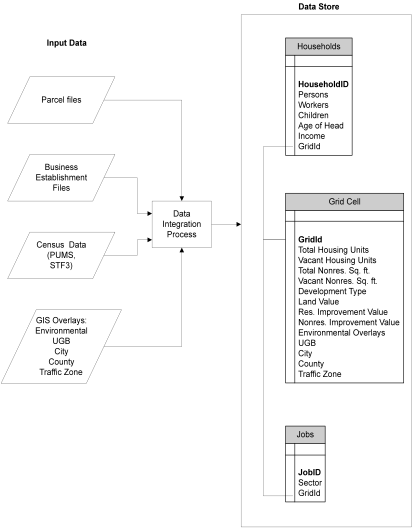
\includegraphics[scale=1.0]{graphics/data-integration.png}
\end{center}
\caption{\label{fig:data-integration}{UrbanSim Data Integration Process, source: Waddell, 2002}}
\end{figure}

\emph{Demographic Transition.}  Interfaces with exogenous (external) information from macroeconomic models that predict the total population, and potentially other aggregate information about population characteristics such as household size and income distributions.  The model component compares these anticipated totals for future years to the UrbanSim household database, to determine how many households of each type must be added or removed from the database in order to be consistent with the external assumptions about total growth or decline of that type of household over the period of one year.

\emph{Economic Transition.}   Serves the same function as the demographic transition component, and adds or removes jobs from the UrbanSim database to achieve consistency with the external assumptions about economic growth or decline in each economic sector over the period of one year.

\emph{Household Relocation.}  Predicts the probability that a household currently located in the region will move over a period of one year. Is sometimes referred to as residential mobility.

\emph{Employment Relocation.}  Predicts the probability that a job in a given sector and location will be moved from that location during a year. Is sometimes referred to as employment mobility.

\emph{Household Location Choice.}     Examines all households that have been added by the demographic transition model, and those that have been selected to move within the current year by the household relocation model, and predicts their location choice from available (existing and vacant) housing units.

\emph{Employment Location Choice.}  Examines all jobs that have been added by the economic transition model, and those that have been predicted to move by the job relocation model, and for each job chooses a location from the available job spaces.

\emph{Real Estate Development Choice.}  Predicts the probability that each location will experience a real estate development event over a one year period, given the characteristics of the location and the market conditions, and if a development event is predicted, predicts the type of development that would occur.

\emph{Land Price.}  Uses location and real estate characteristics to predict land prices at each location, which then informs the location choices of households, firms, and developers in the subsequent time period.

The specification of each of these model components involves the choice of the form of the dependent variable, the functional form of the model, and the independent variables to be included in the model.  A brief compilation of the dependent and independent variables, and the functional form of the key model components in UrbanSim is shown in Table \ref{tab:components}\footnote{This describes a gridcell version of the model system.  The next chapter describes a newer parcel-based version of the model system.}, with the variables used in each model identified by the presence of a symbol in the respective columns.

The model specification leads from the type of process, value, or choice to be predicted. Continuous, numeric, values are typically estimated using linear regression of some type.  See references for the theory of linear regression (Greene, 2003).  In UrbanSim, hedonic, multivariate, regression is used to predict land prices. Many processes can be described as categorical and unordered, for example choice processes such as location choice, development choice, mode choice, route choice, and activity choice. These models are typically specified as probabilistic discrete choice models. There exists a large number of different choice models, with the logit model or a logit model variant as the most common types (Ben-Akiva and Lerman, 1985).

\begin{table}[htp]
\caption{Specification of UrbanSim Model Components}
\label{tab:components}
%\begin{tabular*}{6in}{@{\extracolsep{\fill}} | p{5cm} | p{2cm} | p{2cm} | p{2.5cm} | p{2cm} | }
\begin{tabular}{p{5cm}p{2cm}p{2cm}p{2.5cm}p{2cm}}
\addlinespace
\toprule[1.5pt]
Variable & Household Location Choice & Employment Location Choice & Real Estate Development Choice & Land Price \\
\midrule
Dependent Variable & 150 meter grid cell & 150 meter grid cell & Development event & Log of land price \\
\midrule
Functional Form & Multinomial logit & Multinomial logit & Multinomial logit & Multiple regression \\
\midrule
Independent Variables & & & & \\
\midrule
\addlinespace
Cell: & &  & & \\
\midrule
Land use plan & & & $\bullet$ & $\bullet$ \\
Housing price & $\bullet$ & & $\bullet$ & \\
Housing density & $\bullet$ & & $\bullet$ & $\bullet$ \\
Housing age & $\bullet$ & & $\bullet$ & $\bullet$ \\
\addlinespace
Neighborhood: & & & & \\
\midrule
Distance to urban edge & & & $\bullet$ & $\bullet$ \\
Recent development trends   & & & $\bullet$ &  \\
Land use mix & $\bullet$ & & $\bullet$ & $\bullet$ \\
Land values & & $\bullet$ & $\bullet$ & \\
Jobs by sector  & $\bullet$ & $\bullet$ & & \\
Highways/Arterials  & & $\bullet$ & $\bullet$ & $\bullet$ \\
\addlinespace
Regional:   & & & & \\
\midrule
Job/Population Accessibility & $\bullet$ & $\bullet$ & $\bullet$ & $\bullet$ \\
Vacancy rates   & & & $\bullet$ & $\bullet$ \\
\bottomrule[1.5pt]
\end{tabular}
\end{table}


\subsection{Estimate model parameters}

After the specification of individual models and data preparation the model coefficients must be estimated. The estimation methods are most typically a least squares method, the method of maximum likelihood, or probabilistic simulation in the case when a non-closed form likelihood describes the model.  The least squares methods are widely known and handle a variety of linear and non-linear forms. Many non-linear forms can be converted to linear-in-parameters form and handled with linear regressions, but otherwise non-linear least squares can be used. In addition to single equation models, least squares methods exist for simultaneous systems of equations, most notably seemingly unrelated regression, two-stage least squares, and three-stage least squares. For extensive details on least squares and maximum likelihood methods see references (Greene, 2003).

Probabilistic models are most typically estimated with the method of maximum likelihood, if the likelihood function of the model has a closed form representation. However, for non-closed form likelihoods, methods exist to estimate the coefficients using probabilistic simulation. A popular such method is the Markov-Chain Monte Carlo simulation (Gilks, Richardson and Spiegelhalter, 1996), which is not only robust in the presence of complex model structures, but also provides information on the structure of uncertainty in the joint distribution of the parameter estimates.

\subsection{Calibrate model system}

Following the estimation of the model coefficients, the urban simulation system as a whole must be calibrated. The best way to do this is to have complete data for two time periods. The system is then set up to run from the first time period as its initial condition to the second time period. The system results can then be compared with the data from that time. This allows inaccuracies to be detected and will also potentially show errors in the design. The interaction of the individual models can be calibrated at this stage as desired.

\subsection{Develop Software Application}

Before a model system can be used, it must be implemented in a software application.  In many modelling projects, the software is developed through a customized process that implements a model to the exact specifications of the model and the data used in developing it, but not in a way that facilitates making changes in the data or specification.  These tend to be prototype software applications that rely heavily on `hard-coding' of assumptions about model specifications and data, and are therefore not very general or reusable.  Good software engineering practices can significantly increase the modularity of the software, and improve its performance, ease of maintenance and evolution to address changes in data and model specifications.

Open Source licensing of software is also valuable in increasing the transparency and accessibility of the source code, and has been shown in systems such as Linux to produce extremely robust code.  The UrbanSim software application is based on the Python programming language, and adopts an Open Source licensing approach.  It is freely available on the project web site at http://www.urbansim.org\footnote{UrbanSim was originally implemented in Java, but was converted to Python to make the system easier to use by non-programmers, and to integrate more easily with other software}.

Modularity is increased in the UrbanSim system by forcing all data handling by models to go through a model coordinator.  Data are stored in a standard SQL database, such as MySQL, and are loaded into memory to increase performance.  Simulation results are stored in the database, making the simulation inputs and results accessible from other software applications such as GIS, charting and reporting tools.

\subsection{Validate model system}

To validate the model it is necessary to run it separately on data that was not used to estimate the models or calibrate the system. To do the validation, data is needed from a time period to serve as initial condition and from a later period to serve as a comparison with model predictions. Validation is crucial to give users confidence in the system. Goodness of fit during estimation and calibration is not proof of the quality of the model, since any model can be made to closely match given conditions. It is only when a model is used for different conditions that its predictive power is given.  A historical validation of the UrbanSim model applied to Eugene-Springfield, Oregon has been previously documented (Waddell, 2002).  Practical constraints on creation of historical data for use in validation often preclude the feasibility of historical validation of this sort, but this remains one of the most informative ways to assess the model before putting it into operational use.

\subsection{Operational Use}

The last step is the actual operation of the model. Data is prepared for as recent a time period as possible. The model users then prepare a baseline scenario that contains the assumptions against which other scenarios will be compared.  Generally, for planning purposes, the baseline scenario is a do-nothing or a current-policies set of assumptions that attempt to represent the current set of policies that are in place, with no major policy changes.  Alternative scenarios can then be constructed that contain different assumptions regarding policies and macroeconomic conditions.  Any of the policies to which the model design and specification is sensitive can be included in a scenario.  For example a scenario can include a proposed highway expansion at some future year, or a new light rail system. Also, land policies such as land use plans or urban growth boundaries can be added, removed, or changed, in addition to zoning changes.

Since no model will perfectly predict the future, model predictions are more useful as an indication of the likely direction and magnitude of effects of an alternative scenario when compared to a baseline scenario, than for use as a set of absolute predictions about the future.  In some model applications, information on uncertainty of the outcomes and of the differences between scenarios can be presented, which adds valuable information that can be used to inform policy choices.


\section{Conclusion}

This chapter has sought to explain the context, policy applications, and major design choices in the process of developing an operational urban simulation model, with specific reference to UrbanSim as a case study in model design.  We have argued that careful design at each stage of the process is needed to make the model sensitive to the policies of principal concern, to make the data and computational requirements manageable, to make the model usable by staff and other users with appropriate levels of training, and to fit into the operational practices of the relevant organizations.

To be useful (relevant) in the policy process, model design should carefully integrate the elements discussed here into a design that fits well into a specific institutional and political context, and evolve to adapt to changing conditions.  This introduction to the design process sets the stage for more in-depth discussion of specification and operational issues in model use.

The UrbanSim system is being further developed to adapt to varying data availability, different factors influencing agent choices in locations ranging from newer and rapidly growing U.S. metropolitan areas to older regions with a declining core, as well as issues that arise in metropolitan areas in other parts of the world.  Considerable effort is now being devoted to developing environmental components of the system such as land cover change, and to developing a robust user-interface and tools for visualization and evaluation of policy scenarios.


\section{Bibliography}

Alonso, W. (1964), Location and Land Use. (Cambridge: Harvard University Press.).

Arentze, T., H. Hofman, and H. van Mourik (2000), "Using Decision Tree Induction Systems for Modeling Space-Time Behavior." Geographical Analysis 32, no. 4, pp. 330-350.

Beckman, R. J., K. A. Baggerly, and M. D. McKay. "Creating Synthetic Baseline Populations." Paper presented at the Transportation Research Board Annual Meeting, Washington, D.C., 1995 1995.

Ben-Akiva, M., and S. Lerman (1985), Discrete Choice Analysis: Theory and Application to Travel Demand. (Cambridge, MA: MIT Press.).

Benati, S. (1997), "A Cellular Automaton for the Simulation of Competitive Location." Environment and Planning B: Planning and Design 24, pp. 205 - 218.
Caliper. Transcad. www.caliper.com/tcovu.htm.

Clarke, K., and L. Gaydos (1998), "Loose-Coupling a Cellular Automation Model and Gis: Long-Term Urban Growth Prediction for San Francisco and Washington/Baltimore." Geographical Information Science 12, no. 7, pp. 699-714.

Couclelis, H. (1997), "From Cellular Automata to Urban Models: New Principles for Model Development and Implementation." Environment And Planning B: Planning \& Design 24, pp. 165-174.

de la Barra, T. (1989), Integrated Land Use and Transport Modelling. (Cambridge University Press: Cambridge.).

Deming, W., and F. Stephan (1940), "On a Least Squares Adjustment of a Sampled Frequency Table When the Expected Marginal Totals Are Known." Annals of mathematical statistics, no. 11, pp. 427-444.

Dickey, J. W., and C. Leiner (1983), "Use of Topaz for Transportation-Land Use Planning in a Suburban County." Transportation Research Record 931, pp. 20 - 26.

DiPasquale, D., and W. C. Wheaton (1990), "Housing Market Dynamics and the Future of Housing Prices." 1 - 32: Harvard University; MIT.

Friedman, B., and P. Kahn (1994), "Educating Computer Scientists: Linking the Social and Technical." Communications of the ACM 37, no. 1, pp. 64-70.

Friedman, B., P. Kahn, and A. Borning (2002), "Value Sensitive Design: Theory and Methods." (Seattle: University of Washington). http://www.urbansim.org/papers/vsd-theory-methods-tr.pdf.

Fujita, M., P. Krugman, and A. J. Venables (1999), The Spatial Economy: Cities, Regions and International Trade. (Cambridge: MIT Press.).

Garrett, M., and M. Wachs. "Transportation Planning on Trial: The Clean Air Act and Travel Forecasting -- Introduction \& Conclusions." In Transportation Planning on Trial: The Clean Air Act and Travel Forecasting, 1 - 27; 195 - 223. Thousand Oaks, CA: SAGE Publications, 1996.

Gilks, W. R., S. Richardson, and D. J. Spiegelhalter (1996), Markov Chain Monte Carlo in Practice. (London: Chapman and Hall.).

Goldner, W. (1971), "The Lowry Model Heritage." Journal of the American Institute of Planners 37, no. 2, pp. 100-110.

Greene, W. (2003), Econometric Analysis. 5th ed: Prentice Hall.).

Johnston, R. A. Uplan: Urban Growth Model 2003 [cited June 1 2003]. Available from http://snepmaps.des.ucdavis.edu/uplan.

Klosterman, R. E. (1999), "The What If? Collaborative Planning Support System." Environment and Planning B: Planning and Design 26, pp. 393 - 408.

Landis, J. D. (1994), "The California Urban Futures Model: A New Generation of Metropolitan Simulation Models." Environment and Planning B 21, pp. 399-420.

LANL (2002), "Transportation Analysis Simulation System (Transims) Portland Study Reports." Los Alamos National Laboratory). http://transims.tsasa.lanl.gov/.

Lee, D. (1973), "Requiem for Large Scale Models." Journal of the American Institute of Planners 39, no. 3.

Leontief, W. (1966), Input-Output Economics. (New York: Oxford University Press.).

LUTRAQ (1993), "The Lutraq Alternative/Analysis of Alternatives." (Portland, OR: LUTRAQ, with Cambridge Systematics, Inc., Calthorpe Associates, and Parsons Brinkerhoff Quade and Douglas.

Mackett, R. L. (1992), "Micro Simulation Modelling of Travel and Locational Processes: Testing and Further Development." 1 - 52. (London: Transport Studies Group, University College London.

Marcial Echenique \& Partners Ltd. (1995), "Use of Meplan to Formulate and Evaluate Development Proposals." 1 - 10. (Cambridge: Marcial Echenique \& Partners Ltd.

McFadden, D. "Conditional Logit Analysis of Qualitative Choice Behavior." In Frontiers in Econometrics, edited by P. Zarembka. New York: Academic Press, 1973.

McFadden, D. "Econometric Analysis of Qualitative Response Models." In Handbook of Econometrics, edited by Z. Griliches and M. Inrilligator, 1395-1457. Amsterdam: North Holland, 1984.

McFadden, D. "Structural Discrete Probability Models Derived from Theories of Choice." In Structural Analysis of Discrete Data and Econometric Applications, edited by Charles Manski and Daniel McFadden, 198-272. Cambridge: The MIT Press, 1981.

Mills, E. S. (1967), "An Aggregative Model of Resource Allocation in a Metropolitan Area." American Econometric Review 57, pp. 197-210.

Muth, R. F. (1969), Cities and Housing. (Chicago: University of Chicago Press.).

Noth, M., A. Borning, and P. Waddell (2001), "An Extensible, Modular Architecture for Simulating Urban Development, Transportation, and Environmental Impacts." (Seattle, WA: University of Washington). www.urbansim.org.

Orcutt, G. (1957), "A New Type of Socio-Economic System." Review of Economics and Statistics, no. 58, pp. 773-797.

Orcutt, G., M. Greenberg, J. Korbel, and A. Rivlin (1961), Microanalyis of Socioeconomic Systems: A Simulation Study. (New York: Harper and Row.).

Prastacos, P. (1985), "Urban Development Models for the San Francisco Region: From Plum to Polis." Transportation Research Record, no. 1046, pp. 37-44.

PSRC (1995), "Vision 2020: 1995 Update." (Seattle: Puget Sound Regional Council). www.psrc.org/projects/vision/vision2020.htm.

Putman, S. H. (1983), Integrated Urban Models. (London: Pion.).

Salomon, I., P. Waddell, and M. Wegener. "Sustainable Life Styles? Microsimulation of Household Formation, Housing Choice and Travel Behaviour." In Social Change and Sustainable Transport, edited by W. Black and P. Nijkamp, 125-131. Bloomington, IN: Indiana University Press, 2002.

Schafer, J. (1997), Analysis of Incomplete Multivariate Data, Monographs on Statistics and Applied Probability. (London: Chapman \& Hall.).

Simmonds, D. C. (1999), "The Design of the Delta Land-Use Modelling Package." Environment and Planning B: Planning and Design 26, no. 5, pp. 665 - 684.

Swarm, G. D. Swarm. Santa Fe Institute, Santa Fe, NM. www.swarm.org.

Tesfatsion, L. (2000), "Introduction to the Ce Special Issue on Agent-Based Computational Economics." 1 - 9. (Ames, IA: Department of Economics, Iowa State University.

Waddell, P. (2000), "A Behavioral Simulation Model for Metropolitan Policy Analysis and Planning: Residential Location and Housing Market Components of Urbansim." Environment and Planning B: Planning and Design 27, pp. 247 - 263.

Waddell, P. (2002), "Urbansim: Modeling Urban Development for Land Use, Transportation and Environmental Planning." Journal of the American Planning Association 68, no. 3, pp. 297-314.

Waddell, P., Bhat, E. Ruiter, S. Bekhor, M. Outwater, and E. Schroer (2001), "Review of the Literature and Operational Models: Final Report to the Puget Sound Regional Council on Land Use and Travel Demand Forecasting Models." (Seattle: Puget Sound Regional Council).
 www.psrc.org/datapubs/pubs/model\_review.pdf.

Waddell, P., A. Borning, M. Noth, N. Freier, M. Becke, and G. Ulfarsson (2003), "Urbansim: A Simulation System for Land Use and Transportation." Networks and Spatial Economics 3, pp. 43-67.

Waddell, P., and T. Moore. "Forecasting Demand for Urban Land." In Land Market Monitoring for Smart Urban Growth, 185 - 217. Cambridge, MA: Lincoln Institute for Land Policy, 2001.

Waddell, P., M. Outwater, and C. Bhat (2001), "Recommendations for Integrated Land Use and Travel Models: Final Report to the Puget Sound Regional Council on Land Use and Travel Demand Forecasting Models." (Seattle: Puget Sound Regional Council). www.psrc.org/datapubs/pubs/model\_designrecommendations.pdf.

Waddell, P., E. Schroer, and M. Outwater (2001), "Assessment of Model Requirements: Final Report to the Puget Sound Regional Council on Land Use and Travel Demand Forecasting Models." (Seattle: Puget Sound Regional Council). www.psrc.org/datapubs/pubs/model\_modelrequirements.pdf.

Wegener, M. (1985), "The Dortmund Housing Market Model: A Monte Carlo Simulation of a Regional Housing Market." 144 - 191. (Berlin.

Weiner, E. (1997), "Urban Transportation Planning in the United States: An Historical Overview." 225 - 251. (Washington, D.C.: U. S. Department of Transportation.

White, R., and G. Engelen (1993), "Cellular Automata and Fractal Urban Form: A Cellular Modelling Approach to the Evolution of Urban Land Use Patterns." Environment and Planning A 25, pp. 1175 - 1199.

Wolfram, S. (1984), "Cellular Automata as Models of Complexity." Nature, no. 311, pp. 419-424.
